\begin{figure}[H]\centering
\begin{tikzpicture}
  \node[inner sep=0,anchor=south west] (photo) at (0,0) {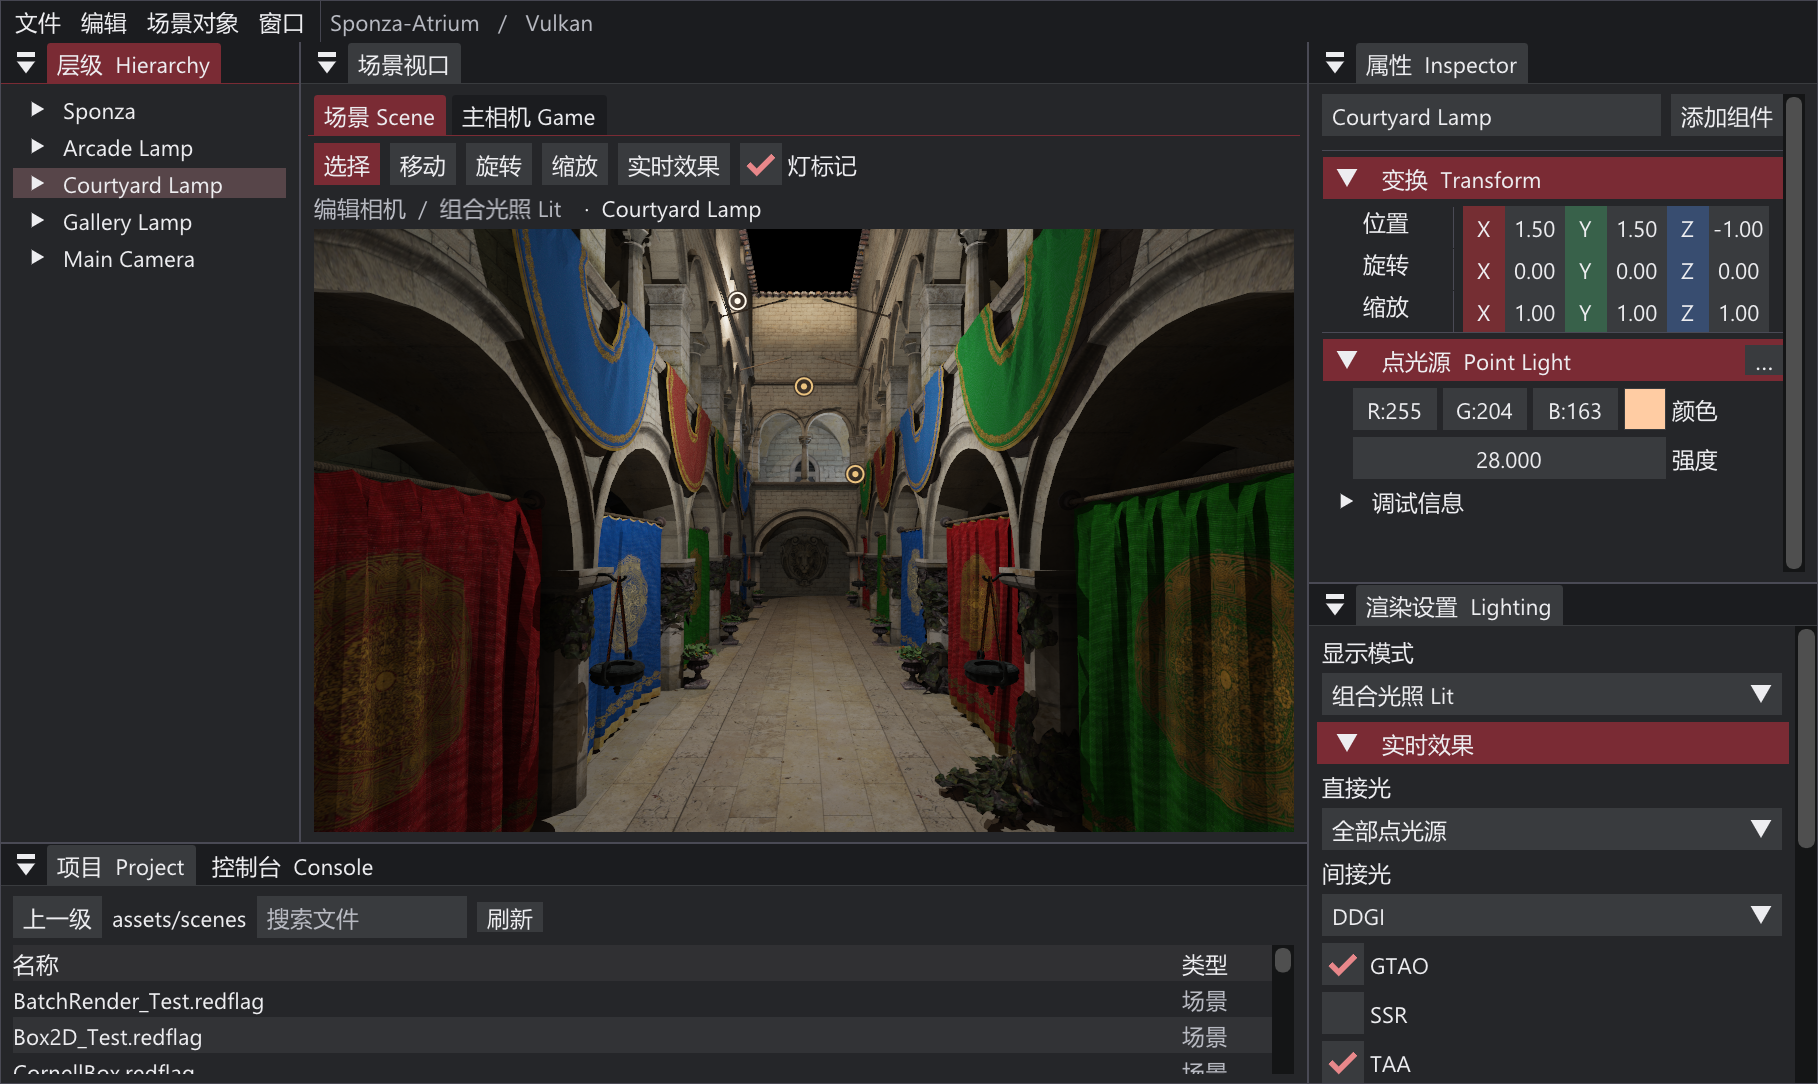
\includegraphics[width=\linewidth]{editor-light-inspector.png}};
  \begin{scope}[x={(photo.south east)},y={(photo.north west)}]
    \tikzset{marker/.style={circle,draw=white,line width=.8pt,fill=Teal,text=white,
      minimum size=5.6mm,inner sep=0pt,font=\sffamily\bfseries\small}}
    \node[marker] at (.135,.83) {1};
    \node[marker] at (.960,.583) {2};
    \node[marker] at (.688,.62) {3};
    \node[marker] at (.644,.16) {4};
  \end{scope}
\end{tikzpicture}
\caption{实际编辑器全窗。按编号可找到层级、属性、场景视口和项目文件。面板停靠位置可调整，本页使用默认布局。}
\end{figure}
